\chapter{Metaheuristics}

\section{What is a metaheuristic?}
A metaheuristic is a problem-solving strategy that consists in a set of steps, a method to be short, with the purpose of finding good solutions to optimization problems.
Unlike heuristics, they are not dependent or tailored to a specific problem in particular, instead they are general problem-solving frameworks applicable to a wide range of cases.
While heuristics are typically very specific on their execution procedure, metaheuristics usually show a higher degree of abstraction, explaining the general approach that should be followed, and leaving the actual details of the implementation to the researcher.
They do not provide guarantees on the optimality of the solution returned, but they aim to find high-quality solutions efficiently.
For this reason they often work in an iteratively manner, repeating a set of steps for a determined amount of times, until some termination condition is met.
Common termination conditions include reaching a convergence criterion in the objective function, finding a solution deemed sufficiently good, or imposing a time limit.
The broad definition of metaheuristics also accounts for the frequent need to adjust parameters for their optimization, which can differ from implementation to implementation.
%This difference with the heuristics can be confirmed also by the ones that we explored in this work. (?)
It is also noticeable that the classic version of both NN and EM are limited in discovering new solutions at each iteration, while metaheuristics usually start from an existing feasible solution, with the objective of improving it.
% Popular metaheuristics that we worked on are \textit{Simulated Annealing}, \textit{Genetic algorithm}, \textit{Tabu Search}, and \textit{Variable Neighborhood Search0}.

\section{2-Opt}
The 2-Opt metaheuristic is a local search method used to improve the solution in optimization problems.
It is based on the idea of iteratively improving a feasible solution of the problem by swapping pairs of edges creating a new solution.
Its name comes from the fact that it replaces two edges each time it optimizes the solution.
%A swap is defined as follows: given $S$ as the set of edges composing the solution and edges $e_{a,b}, e_{c,d} \in S$ a 2-Opt move consists in removing $e_{a,b}, e_{c,d}$ from $S$ and replacing them with edges $e_{a,c}, e_{b,d}$.
A \textbf{swap} is a simple computation in which two edges are removed from a feasible solution and replaced with a new pair of edges such that the solution remains feasible.
Every swap is characterized by their \textbf{offset value}, which represent the quality of the swap and is calculated as the sum of the edges added minus the sum of the edges removed.
Each solution usually allows for a a large number of swaps, however this algorithm is only interested in swaps that allows the overall cost of the tour to be reduced.
These swaps, referred to as \textbf{optimizing swaps} or \textbf{2-Opt moves}, are easily recognized by the fact that their offset is less than zero.
% \begin{definition}
%     Given a solution of TSP $S$, edge $e_1 = (a,b)$ and edge $e_2 = (c,d)$, with $e_1, e_2 \in S$ a \textbf{swap} is the substitution of $e_1$ and $e_2$ with new edges $e_3=(a,c)$ and $e_4=(b,d)$, such that $S$ remains feasible.
% \end{definition}
% Note that there exists only a single combination of edges that allows a swap output to be a feasible solution, otherwise a solution with two subtours is produced, which is an infeasible solution.
% \begin{definition}
%     A 2-Opt move between $e_1 , e_2 \in S$ and $e_3 , e_4 \notin S$ is an \textbf{optimizing swap} or \textbf{2-Opt move} \textit{iff} $C(e_3) + C(e_4) < C(e_1) + C(e_2)$ where $C(e_i)$ is the cost of edge $e_i$ and $S$ is a feasible solution.
% \end{definition}
The first step in the 2-Opt procedure consist in finding a combination of edges that allows for a 2-Opt move.
There are two main approaches to this: the first involves scanning all possible swaps and immediately performing the first 2-Opt move found, while the second involves scanning all possible swaps, identifying the best 2-Opt move, and executing it at the end.
The selected procedure is then repeated until the solution does not allow for any more optimizing swaps.

\begin{figure}[htbp]
    \centering
    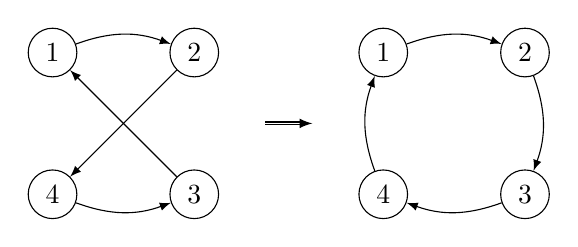
\begin{tikzpicture}[scale=0.6]
        \node[circle, draw, fill=white] (A0) at (0, 0) {1};
        \node[circle, draw, fill=white] (B0) at (3, 0) {2};
        \node[circle, draw, fill=white] (C0) at (3, -3) {3};
        \node[circle, draw, fill=white] (D0) at (0, -3) {4};
    
        \draw[-latex] (A0) to[bend left=20] (B0);
        \draw[-latex] (B0) -- (D0);
        \draw[-latex] (D0) to[bend right=20] (C0);
        \draw[-latex] (C0) -- (A0);
    
        \draw[double,-latex] (4.5,-1.5) -- (5.5,-1.5);
    
        \node[circle, draw, fill=white] (A1) at (7, 0) {1};
        \node[circle, draw, fill=white] (B1) at (10, 0) {2};
        \node[circle, draw, fill=white] (C1) at (10, -3) {3};
        \node[circle, draw, fill=white] (D1) at (7, -3) {4};
    
        \draw[-latex] (A1) to[bend left=20] (B1);
        \draw[-latex] (B1) to[bend left=20] (C1);
        \draw[-latex] (C1) to[bend left=20] (D1);
        \draw[-latex] (D1) to[bend left=20] (A1);
    \end{tikzpicture}
    \caption{2-Opt move}
    \label{fig:2optMoves}
\end{figure}

%Once the edges are swapped the total cost of the tour is recalculated, and if it is lower than the previous cost, the swap is integrated in the solution permanently, or until a better swap involving one of those two edges is found.
%This operation is iterated across all possible pairs of the tour, and is repeated until a time limit is reached, or no further improvements are possible (which involves checking all possible combinations many time, making it infeasible for real-life complex scenarios).
2-Opt can improve significantly a solution, while maintaining an acceptable computational complexity across the board.
Each iteration of 2-Opt is of $O(n^2)$ complexity, while the number of iterations depends both on the quality of the starting solution as well as on the size of the instance itself.
Its main limitation is the fact that due of it being a local search method, it may get stuck in local minima, failing to find the best solution.

\begin{figure}
    \textbf{2-Opt} \\
    \begin{algorithm}[H]
        \SetKwInOut{Input}{Input}
        % \SetKwInOut{Output}{Output}
        \Input{Graph: $G(V,E)$ \newline Cost function: $c_{ij}$ \newline A tour of $G$: $T$}
        % \Output{A better or equaly quality solution}
        \BlankLine
        $finished \gets 0$ \\
        \While{$finished = 0$}{
            $s \gets$ swap with the lowest offset currently in $T$\\
            \eIf{offset($s$) $>$ 0}{
                apply $s$ to $T$
            }{
                $finished \gets 1$
            }
        }
    \end{algorithm}
    \caption{2-Opt algorithm} \label{fig:2OptPseudocode}
\end{figure}

\subsection{Implementation}
% In our implementation of 2-opt we decided to optimize heavily the method using AVX functions rather than multithreading 
% (NOTE: check, and why AVX).
The function that takes care of the application of the metaheuristic is apply2OptBestFix, to which we pass the solution to refine, and will apply the options selected at launch. 
The heart of the algorithm lies in the two specular functions \_2OptBestFix and \_2OptBestFixApprox.
The former will compute the exact edge cost when evaluating edge swaps, considering the actual distance between the points and delivering a more precise result, with the cost of a slower computation, especially for larger instances.
The latter uses an approximated computation of the edges cost and provides a faster iteration time, with the counterpart of possibly producing slightly worse solutions. 
These two methods will iterate over all possible pairs of edges in the tour and compute the potential decrease in total tour length if we were to apply the swap.
The data regarding the best swap found so far, offset of the cost and the edges, is kept in the bestFix struct, to which we will compare each potential swap and which will be then implemented at the end of the iteration.


\subsection{3-Opt}
The 3-opt metaheuristic is an extension of 2-opt, with the difference that it no longer considers two-edge combinations but three-edge combinations instead.
This allows for a larger neighborhood of solutions, and opens to the possibility of escaping situations of local minima that 2-opt might not able to avoid.
It is worth mentioning that while the neighborhood of solutions is larger, escaping from all local minima is not guaranteed and generally not possible with algorithms such as this.
The process is mechanically the same as for 2-opt, with the main difference being the number of nodes involved in a swap and the shape those swap can take.
The concepts of \textbf{swap}, \textbf{optimizing swap} and \textbf{offset value} remain the same as they were in the 2-Opt method.
As shown in \figurename{ \ref{fig:3optMoves}}, the number of possible edge combinations increases significantly.
This, combined with the fact that the possible combinations of three edges are much more numerous than those of two edges, greatly increases computational complexity.
% As shown in figure \ref{fig:3optMoves}, starting from an existing solution, we iteratively consider three edges instead of two, and we change the way they are connected, looking for the one that has lower total cost.
% If a combination is found to improve the total cost of the solution then the swap is implemented, otherwise a different set of three edges is taken into consideration.
% Just as for 2-opt this iterative process can continue until a time limit is reached or until no more improving moves are possible.

\begin{figure}[htbp]
    \centering
    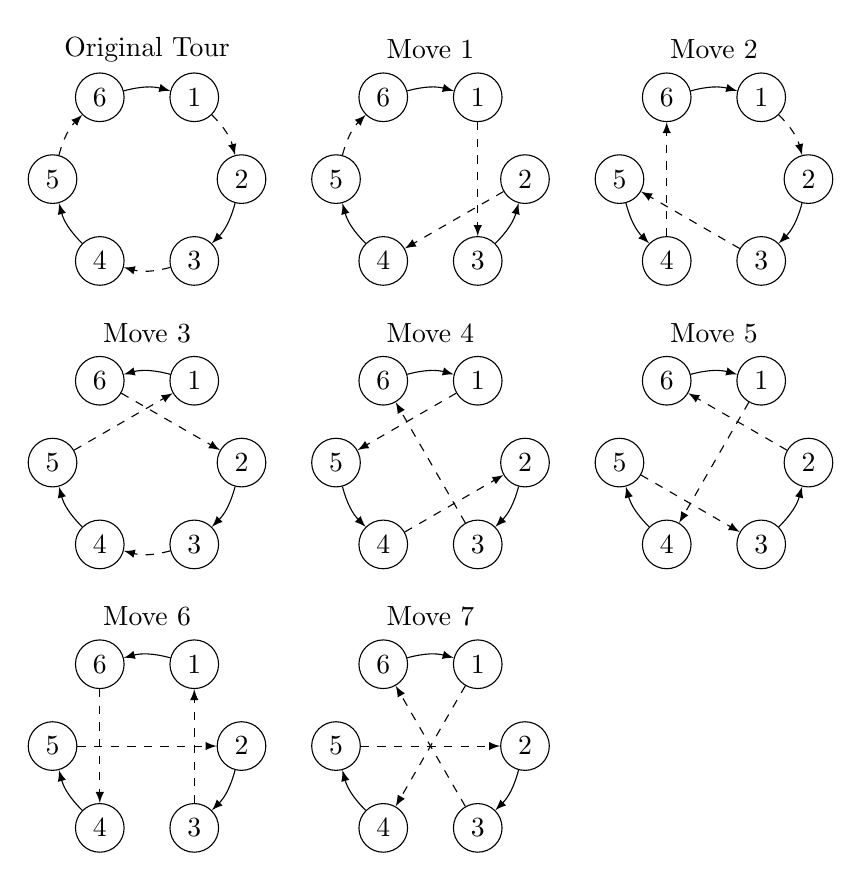
\begin{tikzpicture}[scale=0.6]
        \begin{scope}[shift={(0, 0)}]
            \node at (0, 2.75) {Original Tour};
        
            \node[circle, draw, fill=white] (N1) at ({60 * 2}:2) {6};
            \node[circle, draw, fill=white] (N2) at ({60 * 1}:2) {1};
            \node[circle, draw, fill=white] (N3) at ({60 * 0}:2) {2};
            \node[circle, draw, fill=white] (N4) at ({60 * 5}:2) {3};
            \node[circle, draw, fill=white] (N5) at ({60 * 4}:2) {4};
            \node[circle, draw, fill=white] (N6) at ({60 * 3}:2) {5};
        
            \draw[-latex] (N1) to[bend left=15] (N2);
            \draw[-latex,dashed] (N2) to[bend left=15] (N3);
            \draw[-latex] (N3) to[bend left=15] (N4);
            \draw[-latex,dashed] (N4) to[bend left=15] (N5);
            \draw[-latex] (N5) to[bend left=15] (N6);
            \draw[-latex,dashed] (N6) to[bend left=15] (N1);
        \end{scope}
    
        \begin{scope}[shift={(6, 0)}]
            \node at (0, 2.75) {Move 1};
        
            \node[circle, draw, fill=white] (N1) at ({60 * 2}:2) {6};
            \node[circle, draw, fill=white] (N2) at ({60 * 1}:2) {1};
            \node[circle, draw, fill=white] (N3) at ({60 * 0}:2) {2};
            \node[circle, draw, fill=white] (N4) at ({60 * 5}:2) {3};
            \node[circle, draw, fill=white] (N5) at ({60 * 4}:2) {4};
            \node[circle, draw, fill=white] (N6) at ({60 * 3}:2) {5};
        
            \draw[-latex] (N1) to[bend left=15] (N2);
            \draw[-latex,dashed] (N2) to (N4);
            \draw[-latex,dashed] (N3) to (N5);
            \draw[-latex] (N4) to[bend right=15] (N3);
            \draw[-latex] (N5) to[bend left=15] (N6);
            \draw[-latex,dashed] (N6) to[bend left=15] (N1);
        \end{scope}
    
        \begin{scope}[shift={(12, 0)}]
            \node at (0, 2.75) {Move 2};
        
            \node[circle, draw, fill=white] (N1) at ({60 * 2}:2) {6};
            \node[circle, draw, fill=white] (N2) at ({60 * 1}:2) {1};
            \node[circle, draw, fill=white] (N3) at ({60 * 0}:2) {2};
            \node[circle, draw, fill=white] (N4) at ({60 * 5}:2) {3};
            \node[circle, draw, fill=white] (N5) at ({60 * 4}:2) {4};
            \node[circle, draw, fill=white] (N6) at ({60 * 3}:2) {5};
        
            \draw[-latex] (N1) to[bend left=15] (N2);
            \draw[-latex,dashed] (N2) to[bend left=15] (N3);
            \draw[-latex] (N3) to[bend left=15] (N4);
            \draw[-latex,dashed] (N4) to (N6);
            \draw[-latex,dashed] (N5) to (N1);
            \draw[-latex] (N6) to[bend right=15] (N5);
        \end{scope}
    
        \begin{scope}[shift={(0, -6)}]
            \node at (0, 2.75) {Move 3};
        
            \node[circle, draw, fill=white] (N1) at ({60 * 2}:2) {6};
            \node[circle, draw, fill=white] (N2) at ({60 * 1}:2) {1};
            \node[circle, draw, fill=white] (N3) at ({60 * 0}:2) {2};
            \node[circle, draw, fill=white] (N4) at ({60 * 5}:2) {3};
            \node[circle, draw, fill=white] (N5) at ({60 * 4}:2) {4};
            \node[circle, draw, fill=white] (N6) at ({60 * 3}:2) {5};
        
            \draw[-latex,dashed] (N1) to (N3);
            \draw[-latex] (N2) to[bend right=15] (N1);
            \draw[-latex] (N3) to[bend left=15] (N4);
            \draw[-latex,dashed] (N4) to[bend left=15] (N5);
            \draw[-latex] (N5) to[bend left=15] (N6);
            \draw[-latex,dashed] (N6) to (N2);
        \end{scope}
    
        \begin{scope}[shift={(6, -6)}]
            \node at (0, 2.75) {Move 4};
        
            \node[circle, draw, fill=white] (N1) at ({60 * 2}:2) {6};
            \node[circle, draw, fill=white] (N2) at ({60 * 1}:2) {1};
            \node[circle, draw, fill=white] (N3) at ({60 * 0}:2) {2};
            \node[circle, draw, fill=white] (N4) at ({60 * 5}:2) {3};
            \node[circle, draw, fill=white] (N5) at ({60 * 4}:2) {4};
            \node[circle, draw, fill=white] (N6) at ({60 * 3}:2) {5};
        
            \draw[-latex] (N1) to[bend left=15] (N2);
            \draw[-latex,dashed] (N2) to (N6);
            \draw[-latex] (N3) to[bend left=15] (N4);
            \draw[-latex,dashed] (N4) to (N1);
            \draw[-latex,dashed] (N5) to (N3);
            \draw[-latex] (N6) to[bend right=15] (N5);
        \end{scope}
    
        \begin{scope}[shift={(12, -6)}]
            \node at (0, 2.75) {Move 5};
        
            \node[circle, draw, fill=white] (N1) at ({60 * 2}:2) {6};
            \node[circle, draw, fill=white] (N2) at ({60 * 1}:2) {1};
            \node[circle, draw, fill=white] (N3) at ({60 * 0}:2) {2};
            \node[circle, draw, fill=white] (N4) at ({60 * 5}:2) {3};
            \node[circle, draw, fill=white] (N5) at ({60 * 4}:2) {4};
            \node[circle, draw, fill=white] (N6) at ({60 * 3}:2) {5};
        
            \draw[-latex] (N1) to[bend left=15] (N2);
            \draw[-latex,dashed] (N2) to (N5);
            \draw[-latex,dashed] (N3) to (N1);
            \draw[-latex] (N4) to[bend right=15] (N3);
            \draw[-latex] (N5) to[bend left=15] (N6);
            \draw[-latex,dashed] (N6) to (N4);
        \end{scope}
    
        \begin{scope}[shift={(0, -12)}]
            \node at (0, 2.75) {Move 6};
        
            \node[circle, draw, fill=white] (N1) at ({60 * 2}:2) {6};
            \node[circle, draw, fill=white] (N2) at ({60 * 1}:2) {1};
            \node[circle, draw, fill=white] (N3) at ({60 * 0}:2) {2};
            \node[circle, draw, fill=white] (N4) at ({60 * 5}:2) {3};
            \node[circle, draw, fill=white] (N5) at ({60 * 4}:2) {4};
            \node[circle, draw, fill=white] (N6) at ({60 * 3}:2) {5};
        
            \draw[-latex,dashed] (N1) to (N5);
            \draw[-latex] (N2) to[bend right=15] (N1);
            \draw[-latex] (N3) to[bend left=15] (N4);
            \draw[-latex,dashed] (N4) to (N2);
            \draw[-latex] (N5) to[bend left=15] (N6);
            \draw[-latex,dashed] (N6) to (N3);
        \end{scope}
    
        \begin{scope}[shift={(6, -12)}]
            \node at (0, 2.75) {Move 7};
        
            \node[circle, draw, fill=white] (N1) at ({60 * 2}:2) {6};
            \node[circle, draw, fill=white] (N2) at ({60 * 1}:2) {1};
            \node[circle, draw, fill=white] (N3) at ({60 * 0}:2) {2};
            \node[circle, draw, fill=white] (N4) at ({60 * 5}:2) {3};
            \node[circle, draw, fill=white] (N5) at ({60 * 4}:2) {4};
            \node[circle, draw, fill=white] (N6) at ({60 * 3}:2) {5};
        
            \draw[-latex] (N1) to[bend left=15] (N2);
            \draw[-latex,dashed] (N2) to (N5);
            \draw[-latex] (N3) to[bend left=15] (N4);
            \draw[-latex,dashed] (N4) to (N1);
            \draw[-latex] (N5) to[bend left=15] (N6);
            \draw[-latex,dashed] (N6) to (N3);
        \end{scope}
    
    \end{tikzpicture}
    \caption{3-Opt available moves}
    \label{fig:3optMoves}
\end{figure}

\section{Tabu Search}
Tabu search is a metaheuristic that focuses on escaping local minima.
The idea is to avoid solutions that we know that cannot lead to the global optima.
Let's assume that we alredy have a refined solution, and that we have reached a local minima using the 2-Opt algorithm, let's call this solution $x_i$. 
Trying to further refine it will not provide any improvement, since $x_i$ does not contain any optimizing swap because it was obtained using 2-Opt.
The approach Tabu Search uses to escape from this situation is that of accepting a \textit{bad} move, in other words it performs a swap even if it will cause the cost of the overall cost of the tour to increase.
Therefore a new tour is produced, $x_j$, in the hope that applying 2-Opt once again will yield better solution then $x_i$.
% Hence, the only way to move from this neighborhood of solutions is to accept a \textit{bad} move, in other words we need to perform a swap of some edges that will worsen the solution, generating a new one called $x_{k+1}$, in the hope from it we will be  able to reach a better one.
However there is a high chance that the local search algorithm will turn back from $x_j$ to $x_i$, thus nullifying all the previous efforts.
To avoid this Tabu Seach implements a list called \textbf{tenure} which contains those swaps that are done to escape a local minima.
The tenure works as a list of \textit{forbidden moves} which means that 2-Opt will not be able to perform swaps included within this data structure.
%The way that Tabu Search does this is by implementing a list of edges that cannot be touched, called \textbf{tenure}.
% Any of the edges in this list are \textit{fixed} and we are not allowed to move them with a 2-opt-type move, which forbids a backwards movement from $x_{k+1}$ to $x_k$.
% Logically, without this list, if we were to perform a swap that worsens the solution and we were to  apply 2-opt right after we would just go back to $x_k$, which is the local minima we are trying to escape from.
Of course there are some other considerations to be done on the tenure, involving its size as well as its contents.
Intuitively, the size of this list should be limited, otherwise it might block too many edges and the optimization will become stuck regardless.
Once the list is full, newly introduced \textit{forbidden moves} replace the oldest element in the tenure. 
Another potential improvements regards a detection mechanism on whether the local minima has been escaped or not: by checking if 2-Opt made any improvements on the solution, even while avoiding \textit{forbidden moves}, it is possible to have a rough estimation on wether or not the local optima point has been escaped or not.
Upon detecting a potential escape, removing the oldest element from the tenure in hope of having actually escaped of the local minima.
% This size is called \textit{NOT TENURE}, and could be a fixed amount or it could be adaptive depending on the instance of the problem we are approaching.
% When the list is full, we start replacing the edges in it starting from the older ones.
It is imperative for this procedure to work to its fullest to always keep a copy of the best solution found throughout its execution at all times.
As for the other metaheuristic presented, this process can continue until some termination condition is reached.

\subsection{Implementation(? Maybe talk about the edge locking mechanism)}
TabuSearch is the main method that manages the execution of the tabu algorithm.
After receiving the solution, it sets the tenure size, which is implemented as an array of struct Edge, accordingly to input.
We implemented a check on the value passed for this parameter: if we don't receive any specific size the default value of 2 is set; if we receive a value that is larger of equal to the amount of nodes in 
the instace an error is thrown, since this will lead to the algorithm getting stuck; and lastly, if the value is larger than the 97\% of the 
number of nodes a warning message will indicate the possibility of the method getting stuck and not respecting the time limit.
After this, the function runTabu is launched whithin the threads and takes care of the execution of the metaheuristic, starting from the current best solution (CHECK IF ITS THE PASSED SOLUTION).
The main loop that keeps going until the time limit consists in selecting two random edges in the solution, swapping them and locking one of the two by inserting it into the tenure.
Once we have done that 2-opt is launched to refine the solution, and we keep relaunching it until there are no further improving moves possible, freeing the oldest element in the tenure before relaunching it every time.
A counter is implemented to keep track of the number of iteration in which the method does not find a solution 
that is better than the best one found so far, and when it reaches a threshold the working solution of the thread is resetted back to the best one.

\subsection{Performance}

\begin{figure}[H]
	\centering
	\begin{tikzpicture}
        \begin{axis}[
            xlabel={Cost Ratio},     % AXIS NAME
            %ylabel={Iterations/s Ratio},   % AXIS NAME
            xmin=1, xmax=1.03,       % AXIS LIMITS
            ymin=0, ymax=74,        % AXIS LIMITS
            xtick={},
            ytick=\empty,
            legend style={at={(0.98,0.02)},anchor=south east,legend columns=1}, %MOVE LEGEND HERE
			legend cell align={left},
            %ymajorgrids=true,
            xmajorgrids=true,
            grid style=dashed,
        ]
        
        \addplot[Blue,mark=square,mark size=1.5] table[x=p1cost,y=idx, col sep=semicolon] {csv/tabu.csv}; 
        \addplot[Red,mark=o,mark size=1.5] table[x=p2cost,y=idx, col sep=semicolon] {csv/tabu.csv};
        \addplot[Green,mark=triangle,mark size=1.5] table[x=p3cost,y=idx, col sep=semicolon] {csv/tabu.csv}; 
        \addlegendentry{Tenure size = 1} 
        \addlegendentry{Tenure size = 2}
        \addlegendentry{Tenure size = 3}
            
        \end{axis}
    \end{tikzpicture}
	\caption{Performance comparison between different tenure sizes \label{fig:tabuParmTune}}
\end{figure}

\begin{figure}[H]
	\centering
	\begin{tikzpicture}
        \begin{axis}[
            xlabel={Cost Ratio},     % AXIS NAME
            %ylabel={Iterations/s Ratio},   % AXIS NAME
            xmin=1, xmax=1.082,       % AXIS LIMITS
            ymin=0, ymax=74,        % AXIS LIMITS
            xtick={},
            ytick=\empty,
            legend style={at={(0.98,0.02)},anchor=south east,legend columns=1}, %MOVE LEGEND HERE
			legend cell align={left},
            %ymajorgrids=true,
            xmajorgrids=true,
            grid style=dashed,
        ]
        
        \addplot[Blue,mark=square,mark size=1.5] table[x=startcost,y=idx, col sep=semicolon] {csv/tabu.csv}; 
        \addplot[Red,mark=o,mark size=1.5] table[x=finalcost,y=idx, col sep=semicolon] {csv/tabu.csv};
        \addplot[Green,mark=triangle,mark size=1.5] table[x=optimalcost,y=idx, col sep=semicolon] {csv/tabu.csv}; 
        \addlegendentry{Initial Cost} 
        \addlegendentry{Final Cost}
        \addlegendentry{Optimal Cost}
            
        \end{axis}
    \end{tikzpicture}
	\caption{Performance of with tenure size set to 1 \label{fig:tabuCost}}
\end{figure}

\begin{figure}[H]
	\centering
	\begin{tikzpicture}
        \begin{axis}[
            ylabel={Iterations/s Ratio},     % AXIS NAME
            xlabel={Sorted instances},   % AXIS NAME
            xmin=0, xmax=74,       % AXIS LIMITS
            ymin=1, ymax=1.1,        % AXIS LIMITS
            ytick={},
            xtick=\empty,
            legend style={at={(0.02,0.98)},anchor=north west,,legend columns=1}, %MOVE LEGEND HERE
			legend cell align={left},
            ymajorgrids=true,
            %xmajorgrids=true,
            grid style=dashed,
        ]
        
        \addplot[Blue,mark=square,mark size=1.5] table[y=p1iter,x=idx, col sep=semicolon] {csv/tabu.csv};
        \addplot[Red,mark=o,mark size=1.5] table[y=p2iter,x=idx, col sep=semicolon] {csv/tabu.csv};
        \addplot[Green,mark=triangle,mark size=1.5] table[y=p3iter,x=idx, col sep=semicolon] {csv/tabu.csv};
        \addlegendentry{Tenure size = 1}
        \addlegendentry{Tenure size = 2}
        \addlegendentry{Tenure size = 3} 
            
        \end{axis}
    \end{tikzpicture}
	\caption{Comparison between tabu search parameters and iteration count \label{fig:tabuIters}}
\end{figure}

\section{Variable Neighborhood Search}

Variable Neighborhood Search (VNS) is a technique that explores various neighborhoods within the solution space to seek a potentially optimal solution to a problem.
This metaheuristic closely resembles Tabu Search at a high level of abstraction.
It begins with a feasible solution and explores its neighborhood to identify the best solution within that vicinity before moving on to another neighborhood.
The aim of VNS is to explore different portions of the solution space with the hope of eventually finding the neighborhood of the optimal solution.
% After that we move onto another neighborhood and we explore that one.
The differnce with the previous algorithm is in its behavior on incurring into local minima.
Instead of executing a move that necessarily worsens the solution, VNS addresses the problem by making a completely random move, informally referred to as "kick".
% Indeed there are many type of moves that are suitable for this algorithm, the one we implemented works as follows:
% using $n$ as the magnitude of the "kick", 

While we do this process we keep track of the best solution found so far, and we replace it when a new neighborhood reveals a better minima.
In TSP, to explore the neighborhood of a solution we can use local search algorithms like 2-opt and 3-opt, while to change the neighborhood we perform a swap on a higher amout of edges, five, for instance.
Doing this allows us change the space in which we search for the solution using local search maintaining most of the existing tour untouched.

\begin{figure}[htbp]
    \centering
    \begin{tikzpicture}[scale=1]
        \draw[->] (0,0) -- node[below] {Solution Space} (11,0);
        \draw[->] (0,0) -- node[above,sloped] {Cost} (0,9);
    
        \coordinate (A) at (1, 7);
        \coordinate (B) at (2, 7.5);
        \coordinate (C) at (3, 5);
        \coordinate (D) at (4, 6);
        \coordinate (E) at (5, 3.5);
        \coordinate (F) at (6, 5);
        \coordinate (G) at (7, 1);
        \coordinate (H) at (8, 3.5);
        \coordinate (I) at (9, 4);
        \coordinate (J) at (10, 3.5);
    
        \draw[black,thick] plot [smooth] coordinates {(A) (B) (C) (D) (E) (F) (G) (H) (I) (J)};
    
        \coordinate (P1) at (2.08,7.4);
        \coordinate (P2) at (3.07,5.01);
        \coordinate (P3) at (4.18,5.7);
        \coordinate (P4) at (5.02,3.52);
        \coordinate (P5) at (6.07,4.9);
        \coordinate (P6) at (7.04,1.02);
        
        % Draw jump arrows
        \draw[black,-latex] ([yshift=4]P2) to[out=90, in=180] (3.82,6.4) to[out=0, in=90] ([yshift=4]P3);
        \node[above] at (3.75,6.4) {kick};
        \draw[black,-latex] ([yshift=4]P4) to[out=90, in=180] (5.75,5.5) to[out=0, in=90] ([yshift=4]P5);
        \node[above] at  (5.65,5.5) {kick};
        
        % Comment arrows
        \draw[black,-latex] (2.5,8) -- ([xshift=2,yshift=3.6]P1);
        \node[above right,yshift=0,text width=25mm] at (2.5,8) {\quad Starting \quad Configuration};
        \draw[black,-latex] (6,1) -- ([xshift=-4,yshift=-0.6]P6);
        \node[left,xshift=13,yshift=0,text width=18mm] at (6,1) {\ Global \ Minimum};
        
    
        % Draw points
        \foreach \point in {P1,P2,P3,P4,P5,P6}  {
            \filldraw [black] (\point) circle (2.5pt);
            \filldraw [cyan] (\point) circle (2pt);
        }
    
    \end{tikzpicture}
    \caption{Iteration process of VNS}
    \label{fig:vns}
\end{figure}

VNS balances exploration (through varying neighborhood structures) and exploitation (through local search) to efficiently search the solution space.
The number of edges that we decide to swap can be dependent of the size of the instance, if we were working on a small instance, e.g. 
~50 nodes, swapping more than ten edges could result in a change way too big of the starting solution, worsening it unnecessarily.

\subsection{Implementation(? Maybe talk specifics on how kick works)}
For the implementation of VNS we have the main function VariableNeighborhoodSearch which is in charge of managing the various threads initialization 
and coordination, along with the time management in order to maintain the execution of the algorithm within the time limit provided in input.
Inside the threads we will run parallely the function runVns, which performs the actual algorithm.
The loop inside the threads will start by taking the passed solution and perform a repeating cycle of 2-opt operations and kicks. 2-opt is in charge 
of searching the local space of the solution, while the kick will ensure a traslation to a neighboring search space.
For the kick we implemented a swap of a dynamically chosen amount of edges. We did this to adapt to different scales of instances, since a fixed 
amount of edges swaps (e.g. five each time) could result in a non-effective enough of a neighborhood change for large instances. All the edges involved in the kick are selected randomly.
After each execution of 2-opt the obtained solution will be compared with the saved best solution found so far, and, if the cost is improved, the 
best solution gets updated. Note that the best solution is shared among the threads and its access is managed by mutex.

\subsection{Performance}

\begin{figure}[H]
	\centering
	\begin{tikzpicture}
        \begin{axis}[
            xlabel={Cost Ratio},     % AXIS NAME
            %ylabel={Iterations/s Ratio},   % AXIS NAME
            xmin=1, xmax=1.015,       % AXIS LIMITS
            ymin=0, ymax=74,        % AXIS LIMITS
            xtick={1,1.005,1.01,1.015},
            xticklabel style={/pgf/number format/fixed,/pgf/number format/precision=4},
            ytick=\empty,
            legend style={at={(0.98,0.02)},anchor=south east,legend columns=1}, %MOVE LEGEND HERE
			legend cell align={left},
            %ymajorgrids=true,
            xmajorgrids=true,
            grid style=dashed,
        ]
        
        \addplot[Blue,mark=square,mark size=1.5] table[x=p4_4cost, y=idx, col sep=semicolon] {csv/vns.csv}; 
        \addplot[Red,mark=o,mark size=1.5] table[x=p5_5cost, y=idx, col sep=semicolon] {csv/vns.csv};
        \addplot[Green,mark=triangle,mark size=1.5] table[x=p5_10cost, y=idx, col sep=semicolon] {csv/vns.csv};
        \addplot[Purple,mark=star,mark size=1.5] table[x=p5_20cost, y=idx, col sep=semicolon] {csv/vns.csv};
        \addplot[Dandelion,mark=otimes,mark size=1.5] table[x=p5_40cost, y=idx, col sep=semicolon] {csv/vns.csv};
        \addplot[Black,mark=diamond,mark size=1.5] table[x=p20_40cost, y=idx, col sep=semicolon] {csv/vns.csv};
        \addlegendentry{Kick Config = (4,4)}
        \addlegendentry{Kick Config = (5,5)}
        \addlegendentry{Kick Config = (5,10)}
        \addlegendentry{Kick Config = (5,20)}
        \addlegendentry{Kick Config = (5,40)}
        \addlegendentry{Kick Config = (20,40)}
            
        \end{axis}
    \end{tikzpicture}
	\caption{Performance comparison between different KICKs configurations \label{fig:vnsParmTune}}
\end{figure}

\begin{figure}[H]
	\centering
	\begin{tikzpicture}
        \begin{axis}[
            xlabel={Cost Ratio},     % AXIS NAME
            %ylabel={Iterations/s Ratio},   % AXIS NAME
            xmin=1, xmax=1.082,       % AXIS LIMITS
            ymin=0, ymax=74,        % AXIS LIMITS
            xtick={},
            ytick=\empty,
            legend style={at={(0.98,0.02)},anchor=south east,legend columns=1}, %MOVE LEGEND HERE
			legend cell align={left},
            %ymajorgrids=true,
            xmajorgrids=true,
            grid style=dashed,
        ]
        
        \addplot[Blue,mark=square,mark size=1.5] table[x=startcost,y=idx, col sep=semicolon] {csv/vns.csv}; 
        \addplot[Red,mark=o,mark size=1.5] table[x=finalcost,y=idx, col sep=semicolon] {csv/vns.csv};
        \addplot[Green,mark=triangle,mark size=1.5] table[x=optimalcost,y=idx, col sep=semicolon] {csv/vns.csv}; 
        \addlegendentry{Initial Cost} 
        \addlegendentry{Final Cost}
        \addlegendentry{Optimal Cost}
            
        \end{axis}
    \end{tikzpicture}
	\caption{Performance of with KICK configuration set to (5,10) \label{fig:vnsCost}}
\end{figure}

\begin{figure}[H]
	\centering
	\begin{tikzpicture}
        \begin{axis}[
            ylabel={Iterations/s Ratio},     % AXIS NAME
            xlabel={Sorted instances},   % AXIS NAME
            xmin=0, xmax=74,       % AXIS LIMITS
            ymin=1, ymax=18,        % AXIS LIMITS
            ytick={1,2,4,6,8,10,12,14,16},
            xtick=\empty,
            legend style={at={(0.02,0.98)},anchor=north west,,legend columns=1}, %MOVE LEGEND HERE
			legend cell align={left},
            ymajorgrids=true,
            %xmajorgrids=true,
            grid style=dashed,
        ]
        
        \addplot[Blue,mark=square,mark size=1.5] table[y=p4_4iter, x=idx, col sep=semicolon] {csv/vns.csv}; 
        \addplot[Red,mark=o,mark size=1.5] table[y=p5_5iter, x=idx, col sep=semicolon] {csv/vns.csv};
        \addplot[Green,mark=triangle,mark size=1.5] table[y=p5_10iter, x=idx, col sep=semicolon] {csv/vns.csv};
        \addplot[Purple,mark=star,mark size=1.5] table[y=p5_20iter, x=idx, col sep=semicolon] {csv/vns.csv};
        \addplot[Dandelion,mark=otimes,mark size=1.5] table[y=p5_40iter, x=idx, col sep=semicolon] {csv/vns.csv};
        \addplot[Black,mark=diamond,mark size=1.5] table[y=p20_40iter, x=idx, col sep=semicolon] {csv/vns.csv};
        \addlegendentry{Kick Config = (4,4)}
        \addlegendentry{Kick Config = (5,5)}
        \addlegendentry{Kick Config = (5,10)}
        \addlegendentry{Kick Config = (5,20)}
        \addlegendentry{Kick Config = (5,40)}
        \addlegendentry{Kick Config = (20,40)}
            
        \end{axis}
    \end{tikzpicture}
	\caption{Comparison between VNS parameters in speed \label{fig:vnsIters}}
\end{figure}


\section{Simulated Annealing}
Simulated Annealing (SA) is a probabilistic metaheuristic inspired by the annealing process in metallurgy, where a material in heated
and then slowly cooled in order to improve its quality. The main parameter for this method is in fact called \textit{temperature}.
The value of this parameter indicates the probaility for which we allow our method to accept bad moves (e.g. swap two edges that 
don't improve the solution cost). Initially this parameter is set high, which allows for a greater exploration of the solution space.
At every iteration this parameter is scaled down (by a factor of $0.9$ or $0.95$ for example), gradually allowing for less and less 
bad moves, restricting the search space. 

\begin{figure}[H]
    \centering
    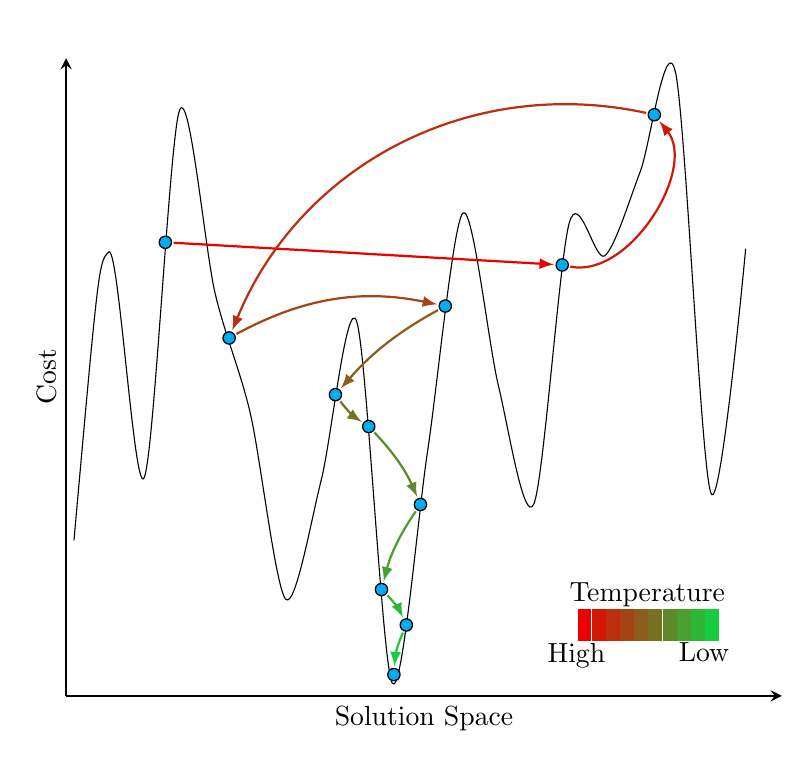
\begin{tikzpicture}
		[scale=0.9,shorten <=3pt,shorten >=3pt,>=stealth]

        \draw[thick,->,shorten <=0pt,shorten >=0pt,>=stealth] (-0.1,1) -- node[below] {Solution Space} (10,1);
        \draw[thick,->,shorten <=0pt,shorten >=0pt,>=stealth] (-0.1,1) -- node[above,sloped] {Cost} (-0.1,10);

		\draw[black,] plot [smooth] coordinates {(0,3.076)(0.5,7.263)(1,4.076)(1.5,9.263)(2,6.689)(2.5,4.981)(3,2.362)(3.5,4.046)(4,6.282)(4.5,1.183)(5,4.45)(5.5,7.813)(6,5.376)(6.5,3.708)(7,7.675)(7.5,7.209)(8,8.394)(8.5,9.791)(9,3.856)(9.5,7.428)};

        \coordinate (P1) at (1.3,7.4);
        \coordinate (P2) at (6.9,7.08);
        \coordinate (P3) at (8.2,9.2);
        \coordinate (P4) at (2.2,6.05);
        \coordinate (P5) at (5.25,6.5);
        \coordinate (P6) at (3.7,5.25);
        \coordinate (P7) at (4.17,4.8);
        \coordinate (P8) at (4.9,3.7);
        \coordinate (P9) at (4.35,2.5);
        \coordinate (P10) at (4.7,2);
        \coordinate (P11) at (4.525,1.3);
              
        \foreach \point in {P1,P2,P3,P4,P5,P6,P7,P8,P9,P10,P11}  {
            \filldraw [black] (\point) circle (2.5pt);
            \filldraw [cyan] (\point) circle (2pt);
        }

        \definecolor{C1}{RGB}{235, 0, 0}
        \definecolor{C2}{RGB}{211, 23, 7}
        \definecolor{C3}{RGB}{188, 46, 14}
        \definecolor{C4}{RGB}{164, 68, 20}
        \definecolor{C5}{RGB}{141, 91, 27}
        \definecolor{C6}{RGB}{118, 114, 34}
        \definecolor{C7}{RGB}{94, 137, 41}
        \definecolor{C8}{RGB}{71, 160, 48}
        \definecolor{C9}{RGB}{47, 182, 54}
        \definecolor{C10}{RGB}{24, 205, 61}

		\draw[-latex,color=C1,thick] (P1) to (P2);
		\draw[-latex,color=C2,thick] (P2) to[bend right=70] (P3);
		\draw[-latex,color=C3,thick] (P3) to[bend right=40] (P4);
		\draw[-latex,color=C4,thick] (P4) to[bend left=20] (P5);
		\draw[-latex,color=C5,thick] (P5) to[bend right=10] (P6);
		\draw[-latex,color=C6,thick] (P6) to[bend right=10] (P7);
		\draw[-latex,color=C7,thick] (P7) to[bend left=10] (P8);
		\draw[-latex,color=C8,thick] (P8) to[bend right=10] (P9);
		\draw[-latex,color=C9,thick] (P9) to[bend left=10] (P10);
		\draw[-latex,color=C10,thick] (P10) to[bend right=10] (P11);

        \draw[line width=4mm, color=C1] (7,2) -- ++(0.43,0);
        \draw[line width=4mm, color=C2] (7.2,2) -- ++(0.43,0);
        \draw[line width=4mm, color=C3] (7.4,2) -- ++(0.43,0);
        \draw[line width=4mm, color=C4] (7.6,2) -- ++(0.43,0);
        \draw[line width=4mm, color=C5] (7.8,2) -- ++(0.43,0);
        \draw[line width=4mm, color=C6] (8,2) -- ++(0.43,0);
        \draw[line width=4mm, color=C7] (8.2,2) -- ++(0.43,0);
        \draw[line width=4mm, color=C8] (8.4,2) -- ++(0.43,0);
        \draw[line width=4mm, color=C9] (8.6,2) -- ++(0.43,0);
        \draw[line width=4mm, color=C10] (8.8,2) -- ++(0.43,0);

        \node[above,yshift=3] at (8.1,2) {Temperature};
        \node[below,yshift=-3] at (7.1,2) {High};
        \node[below,yshift=-3] at (8.9,2) {Low};

    \end{tikzpicture}
    \caption{Iteration process of Simulated Annealing}
    \label{fig:sa}
\end{figure}

\subsection{Implementation}
For the implementation of Simulated Annealing we decided to set up a number of constants in order to be able to tweak the parameters of the 
method in input. Fixed parameters can work fine for instances of similar magnitude, but to allow for a good execution for both large and small 
instances we thought this was the best approach. The parameteres we are talking are:

\begin{enumerate}
    \item SAME\_TEMP\_MOVES\_THRESHOLD: Number of moves to perform before reducing the temperature.
    \item TEMPERATURE\_MULTIPLIER: Factor by which the temperature is multiplied to decrease it; should be slightly less than 1.
    \item STOP\_TEMP: Temperature at which SA stops and runs a 2-opt algorithm for further optimization.
    \item MAX\_TRIES\_FUNC(n): Function to determine the maximum number of move attempts before increasing the temperature.
    \item USE\_RATIO\_ACCEPTANCE: A macro to toggle the use of ratio-based acceptance criteria.
\end{enumerate}


The execution of this metaheuristic is managed by the function SimulatedAnnealing, that mainly sets up the desired number of threads and launches them 
on the function runSimulatedAnnealing. 
The actual algorithm is then executed parallely within each thread until the time limit is reached. During this time we perform moves up to what we 
specified on STOP\_TEMP, then we will launch the 2-opt metaheuristic to further refine the solution within its space. 
After a certain amount of non-improving iterations, we restart the method from the best solution found so far, which we are keeping track at all 
times and is accessible by the use of a mutex by all threads. This is to fully use the time provided in the time limit, and to give the method more chances to escape a local minima.

\subsection{Performance}

\begin{figure}[H]
	\centering
	\begin{tikzpicture}
        \begin{axis}[
            xlabel={Improvement Ratio},     % AXIS NAME
            %ylabel={Iterations/s Ratio},   % AXIS NAME
            xmin=1, xmax=1.08,       % AXIS LIMITS
            ymin=0, ymax=69,        % AXIS LIMITS
            xtick={},
            xticklabel style={/pgf/number format/fixed,/pgf/number format/precision=4},
            ytick=\empty,
            legend style={at={(0.98,0.02)},anchor=south east,legend columns=1}, %MOVE LEGEND HERE
			legend cell align={left},
            %ymajorgrids=true,
            xmajorgrids=true,
            grid style=dashed,
        ]
        
        \addplot[Blue,mark=square,mark size=1.5] table[x=improve3, y=idx, col sep=semicolon] {csv/annealing.csv}; 
        \addplot[Red,mark=o,mark size=1.5] table[x=improve6, y=idx, col sep=semicolon] {csv/annealing.csv};
        \addplot[Green,mark=triangle,mark size=1.5] table[x=improve9, y=idx, col sep=semicolon] {csv/annealing.csv};
        \addplot[Purple,mark=star,mark size=1.5] table[x=aimprove3, y=idx, col sep=semicolon] {csv/annealing.csv};
        \addplot[Dandelion,mark=otimes,mark size=1.5] table[x=aimprove6, y=idx, col sep=semicolon] {csv/annealing.csv};
        \addplot[Black,mark=diamond,mark size=1.5] table[x=aimprove9, y=idx, col sep=semicolon] {csv/annealing.csv};
        \addlegendentry{Temp = 3}
        \addlegendentry{Temp = 6}
        \addlegendentry{Temp = 9}
        \addlegendentry{Temp = 3 (alt acceptance)}
        \addlegendentry{Temp = 6 (alt acceptance)}
        \addlegendentry{Temp = 9 (alt acceptance)}
            
        \end{axis}
    \end{tikzpicture}
	\caption{Performance comparison between different Annealing configurations in terms of $\frac{final\_cost}{start\_cost}$ (Higher is better)}
    \label{fig:annealingParmTune}
\end{figure}

\begin{figure}[H]
	\centering
	\begin{tikzpicture}
        \begin{axis}[
            ylabel={Iterations/s Ratio},     % AXIS NAME
            xlabel={Sorted instances},   % AXIS NAME
            xmin=0, xmax=69,       % AXIS LIMITS
            ymin=1, ymax=2.5,        % AXIS LIMITS
            ytick={},
            xtick=\empty,
            legend style={at={(0.02,0.98)},anchor=north west,,legend columns=1}, %MOVE LEGEND HERE
			legend cell align={left},
            ymajorgrids=true,
            %xmajorgrids=true,
            grid style=dashed,
        ]
        
        
        \addplot[Blue,mark=square,mark size=1.5] table[y=iter3, x=idx, col sep=semicolon] {csv/annealing.csv}; 
        \addplot[Red,mark=o,mark size=1.5] table[y=iter6, x=idx, col sep=semicolon] {csv/annealing.csv};
        \addplot[Green,mark=triangle,mark size=1.5] table[y=iter9, x=idx, col sep=semicolon] {csv/annealing.csv};
        \addplot[Purple,mark=star,mark size=1.5] table[y=aiter3, x=idx, col sep=semicolon] {csv/annealing.csv};
        \addplot[Dandelion,mark=otimes,mark size=1.5] table[y=aiter6, x=idx, col sep=semicolon] {csv/annealing.csv};
        \addplot[Black,mark=diamond,mark size=1.5] table[y=aiter9, x=idx, col sep=semicolon] {csv/annealing.csv};
        \addlegendentry{Temp = 3}
        \addlegendentry{Temp = 6}
        \addlegendentry{Temp = 9}
        \addlegendentry{Temp = 3 (alt acceptance)}
        \addlegendentry{Temp = 6 (alt acceptance)}
        \addlegendentry{Temp = 9 (alt acceptance)}
            
        \end{axis}
    \end{tikzpicture}
	\caption{Comparison between Simulated Annealing parameters in speed}
    \label{fig:annealingIters}
\end{figure}

There does not seems to be any favorable configuration (next graph uses temp=6 data (no alt edge acceptance))

\begin{figure}[H]
	\centering
	\begin{tikzpicture}
        \begin{axis}[
            xlabel={Cost Ratio},     % AXIS NAME
            %ylabel={Iterations/s Ratio},   % AXIS NAME
            xmin=1, xmax=1.082,       % AXIS LIMITS
            ymin=0, ymax=69,        % AXIS LIMITS
            xtick={},
            ytick=\empty,
            legend style={at={(0.98,0.02)},anchor=south east,legend columns=1}, %MOVE LEGEND HERE
			legend cell align={left},
            %ymajorgrids=true,
            xmajorgrids=true,
            grid style=dashed,
        ]
        
        \addplot[Blue,mark=square,mark size=1.5] table[x=startcost,y=idx, col sep=semicolon] {csv/annealing.csv}; 
        \addplot[Red,mark=o,mark size=1.5] table[x=finalcost,y=idx, col sep=semicolon] {csv/annealing.csv};
        \addplot[Green,mark=triangle,mark size=1.5] table[x=optimalcost,y=idx, col sep=semicolon] {csv/annealing.csv}; 
        \addlegendentry{Initial Cost} 
        \addlegendentry{Final Cost}
        \addlegendentry{Optimal Cost}
            
        \end{axis}
    \end{tikzpicture}
	\caption{Overall Performance of Simulated Annealing}
    \label{fig:annealingCost}
\end{figure}

\section{Genetic}
\subsection{Implementation}
In a similar fashion of the algorithms previously presented, for the Genetic Algorithm we also have a main method, GeneticAlgorithm, that is in 
charge of managing the creation and synchronization of the various threads. The actual algorithm is performed then within each thread by the function runGenetic.
A series macros are used throughout the code to configure the genetic algorithm's behavior without hardcoding values. For example, the population 
size and the number of genetic operations (crossover, mutation, reintroduction) are dynamically calculated based on the instance parameters using 
POPULATION\_SIZE, CROSSOVER\_AMOUNT, MUTATION\_AMOUNT and REINTRO\_AMOUNT. 

\subsection{Performance}

\begin{itemize}
    \item \textbf{Config 1}: Population = 50, Crossover = 10, Mutation = 10, Reintro =  5
    \item \textbf{Config 1}: Population = 50, Crossover = 20, Mutation = 20, Reintro =  5
    \item \textbf{Config 1}: Population = 100, Crossover = 50, Mutation = 20, Reintro = 20
    \item \textbf{Config 1}: Population = 100, Crossover = 20, Mutation = 50, Reintro = 20
    \item \textbf{Config 1}: Population = 100, Crossover = 40, Mutation = 40, Reintro = 10
\end{itemize}

\begin{figure}[H]
	\centering
	\begin{tikzpicture}
        \begin{axis}[
            xlabel={Cost Ratio},     % AXIS NAME
            %ylabel={Iterations/s Ratio},   % AXIS NAME
            xmin=1, xmax=2.7,       % AXIS LIMITS
            ymin=0, ymax=42,        % AXIS LIMITS
            xtick={},
            xticklabel style={/pgf/number format/fixed,/pgf/number format/precision=4},
            ytick=\empty,
            legend style={at={(0.98,0.02)},anchor=south east,legend columns=1}, %MOVE LEGEND HERE
			legend cell align={left},
            %ymajorgrids=true,
            xmajorgrids=true,
            grid style=dashed,
        ]
        
        \addplot[Blue,mark=square,mark size=1.5] table[x=cost_50_10_10_5, y=idx, col sep=semicolon] {csv/genetic.csv}; 
        \addplot[Red,mark=o,mark size=1.5] table[x=cost_50_20_20_5, y=idx, col sep=semicolon] {csv/genetic.csv};
        \addplot[Green,mark=triangle,mark size=1.5] table[x=cost_100_50_20_20, y=idx, col sep=semicolon] {csv/genetic.csv};
        \addplot[Purple,mark=star,mark size=1.5] table[x=cost_100_20_50_20, y=idx, col sep=semicolon] {csv/genetic.csv};
        \addplot[Dandelion,mark=otimes,mark size=1.5] table[x=cost_100_40_40_10, y=idx, col sep=semicolon] {csv/genetic.csv};
        \addlegendentry{Config 1}
        \addlegendentry{Config 2}
        \addlegendentry{Config 3}
        \addlegendentry{Config 4}
        \addlegendentry{Config 5}
            
        \end{axis}
    \end{tikzpicture}
	\caption{Performance comparison between different Genetic configurations}
    \label{fig:geneticParmTune}
\end{figure}

\begin{figure}[H]
	\centering
	\begin{tikzpicture}
        \begin{axis}[
            ylabel={Iterations/s Ratio},     % AXIS NAME
            xlabel={Sorted instances},   % AXIS NAME
            xmin=0, xmax=42,       % AXIS LIMITS
            ymin=1, ymax=8,        % AXIS LIMITS
            ytick={},
            xtick=\empty,
            legend style={at={(0.02,0.98)},anchor=north west,,legend columns=1}, %MOVE LEGEND HERE
			legend cell align={left},
            ymajorgrids=true,
            %xmajorgrids=true,
            grid style=dashed,
        ]
        
        
        \addplot[Blue,mark=square,mark size=1.5] table[y=iter_50_10_10_5, x=idx, col sep=semicolon] {csv/genetic.csv}; 
        \addplot[Red,mark=o,mark size=1.5] table[y=iter_50_20_20_5, x=idx, col sep=semicolon] {csv/genetic.csv};
        \addplot[Green,mark=triangle,mark size=1.5] table[y=iter_100_50_20_20, x=idx, col sep=semicolon] {csv/genetic.csv};
        \addplot[Purple,mark=star,mark size=1.5] table[y=iter_100_20_50_20, x=idx, col sep=semicolon] {csv/genetic.csv};
        \addplot[Dandelion,mark=otimes,mark size=1.5] table[y=iter_100_40_40_10, x=idx, col sep=semicolon] {csv/genetic.csv};
        \addlegendentry{Config 1}
        \addlegendentry{Config 2}
        \addlegendentry{Config 3}
        \addlegendentry{Config 4}
        \addlegendentry{Config 5}
            
        \end{axis}
    \end{tikzpicture}
	\caption{Comparison between Genetic configurations in speed}
    \label{fig:geneticIters}
\end{figure}

\begin{figure}[H]
	\centering
	\begin{tikzpicture}
        \begin{axis}[
            xlabel={Cost Ratio},     % AXIS NAME
            %ylabel={Iterations/s Ratio},   % AXIS NAME
            xmin=1, xmax=17,       % AXIS LIMITS
            ymin=0, ymax=42,        % AXIS LIMITS
            xtick={},
            ytick=\empty,
            legend style={at={(0.98,0.02)},anchor=south east,legend columns=1}, %MOVE LEGEND HERE
			legend cell align={left},
            %ymajorgrids=true,
            xmajorgrids=true,
            grid style=dashed,
        ]
        
        \addplot[Red,mark=o,mark size=1.5] table[x=finalcost,y=idx, col sep=semicolon] {csv/genetic.csv}; 
        \addplot[Green,mark=triangle,mark size=1.5] table[x=optimalcost,y=idx, col sep=semicolon] {csv/genetic.csv};
        \addlegendentry{Final Cost}
        \addlegendentry{Optimal Cost}
            
        \end{axis}
    \end{tikzpicture}
	\caption{Overall Performance of Genetic}
    \label{fig:geneticCost}
\end{figure}

\section{Comparison}

\begin{figure}[H]
	\centering
	\begin{tikzpicture}
        \begin{axis}[
            xlabel={Cost Ratio},     % AXIS NAME
            %ylabel={Iterations/s Ratio},   % AXIS NAME
            xmin=1, xmax=1.05,       % AXIS LIMITS
            ymin=0, ymax=74,        % AXIS LIMITS
            xtick={},
            xticklabel style={/pgf/number format/fixed,/pgf/number format/precision=4},
            ytick=\empty,
            legend style={at={(0.98,0.02)},anchor=south east,legend columns=1}, %MOVE LEGEND HERE
			legend cell align={left},
            %ymajorgrids=true,
            xmajorgrids=true,
            grid style=dashed,
        ]
        
        \addplot[Blue,mark=square,mark size=1.5] table[x=tabu_1, y=idx, col sep=semicolon] {csv/cmp_metaheuristics.csv}; 
        \addplot[Red,mark=o,mark size=1.5] table[x=vns_5-10, y=idx, col sep=semicolon] {csv/cmp_metaheuristics.csv};
        \addplot[Green,mark=triangle,mark size=1.5] table[x=annealing_std6, y=annealing_idx, col sep=semicolon] {csv/cmp_metaheuristics.csv};
        % \addplot[Purple,mark=star,mark size=1.5] table[x=genetic, y=genetic_idx, col sep=semicolon] {csv/cmp_metaheuristics.csv};
        \addlegendentry{tabu}
        \addlegendentry{VNS}
        \addlegendentry{Annealing}
        % \addlegendentry{Genetic}
            
        \end{axis}
    \end{tikzpicture}
	\caption{Comparsion between all metaheuristics with best parameters found}
    \label{fig:metacmp}
\end{figure}